\chapter{共振 (Resonances)}\label{ch:resonance}

在前一章我们详细讨论了 Jost 函数 $f_\ell(p)$ 与分波 $S$ 矩阵元
$\mathsf{s}_\ell(p)=f_\ell(-p)/f_\ell(p)$ 在复 $p$ 平面上的解析性质，并指出
束缚态对应于 Jost 函数在正虚轴 $\Im p>0$ 上的零点（亦即 $\mathsf{s}_\ell$ 的极点）。
本章把这一框架推广到下半平面 $\Im p<0$：那里同样可能存在 $f_\ell$ 的零点，
它们对应于 $\mathsf{s}_\ell(p)$ 的极点，称为\textbf{共振极点 (resonance poles)}。
共振对应的能量 $E_R-\rmi\Gamma/2$ 位于复能量平面的下半叶（第二黎曼叶），
直接产生散射截面在 $E\approx E_R$ 处的尖锐峰，在时间演化中表现为
寿命 $\tau\sim\hbar/\Gamma$ 的亚稳态 (quasi-stationary state)。

参考资料：本章基于 Zhiguang 讲义第 12 讲，
并以 Taylor《Scattering Theory》第 13 章作为补充。

\section{共振的现象学}

实验上经常观测到散射截面 $\sigma(E)$ 作为入射能量 $E$ 的函数时
出现\emph{尖锐而隔离}的峰，例如：
\begin{itemize}
  \item 中子打铱核 (neutrons off iridium)：在 $\sim 1\,\mathrm{eV}$ 附近出现一系列
    宽度为 $\mathrm{meV}$ 量级的尖峰；
  \item $\pi^+$ 介子打质子 (pions off protons)：在总能量
    $\sim 1.2\,\mathrm{GeV}$ 处出现著名的 $\Delta(1232)$ 共振峰，
    宽度约 $100\,\mathrm{MeV}$。
\end{itemize}
这种现象意味着：在散射过程中，对某些特殊能量 $E_R$，
入射粒子与靶被短暂地俘获，形成一个接近束缚态的"亚稳态"
(quasi-stationary state)；该态会在有限寿命 $\tau$ 内衰变回散射末态。
当入射能量恰好接近 $E_R$ 时散射振幅被显著放大，从而使截面剧烈变化。

回忆束缚态对应 $\Im p>0$ 虚轴上 $f_\ell(p)$ 的零点 / $\mathsf{s}_\ell(p)$ 的极点。
后面我们将看到，共振对应 $\Im p<0$ 时 $f_\ell(p)$ 的零点 /
$\mathsf{s}_\ell(p)$ 的极点。

\begin{definition}[共振极点]\label{def:res-pole}
  设分波 $S$ 矩阵元 $\mathsf{s}_\ell(p)$ 可解析延拓至 $\Im p<0$ 的下半平面。
  若 $\mathsf{s}_\ell(p)$ 在 $\bar p=p_R-\rmi p_I$（$p_R>0,\;p_I>0$）处有一个
  孤立的极点，则称之为一个 \emph{共振极点}，对应的复能量
  \begin{equation}
    \bar E=\frac{\bar p^{\,2}}{2m}=E_R-\rmi\frac{\Gamma}{2},\qquad
    E_R=\frac{p_R^2-p_I^2}{2m},\quad \Gamma=\frac{2 p_R p_I}{m},
  \end{equation}
  其中 $E_R>0$ 称为\emph{共振能量}，$\Gamma>0$ 称为\emph{共振宽度}，
  对应的寿命为 $\tau=1/\Gamma$（自然单位 $\hbar=1$）。
\end{definition}

\section{$\mathsf{s}_\ell$ 矩阵的下半平面极点与共振相移}

设 $f_\ell(p)$ 可被解析延拓至 $\Im p<0$ 的下半 $p$-平面，
则在接近实轴处 $\bar p=p_R-\rmi p_I$（$p_R>0,p_I>0$）一般会有
一个零点。由 $\mathsf{s}_\ell(p)=f_\ell(-p)/f_\ell(p)$ 知 $\bar p$
对应 $\mathsf{s}_\ell(p)$ 的极点。我们考察 $f_\ell$ 在该点附近的行为
（假设是单零点且离实轴足够近）：
\begin{equation}
  f_\ell(p)\simeq\left(\frac{\rmd f_\ell}{\rmd p}\right)_{\bar p}(p-\bar p)
  ,\qquad \bar p=p_R-\rmi p_I.
\end{equation}

\subsection{零点处的"波函数"}

回顾上一章 Jost 解的归一化关系，在零点 $\bar p$ 处约化波函数
满足
\begin{equation}
  \phi^+_{\ell,\bar p}(r)\propto f_\ell(-\bar p)\chi^+_{\ell,\bar p}(r),
  \qquad \chi^+_{\ell,\bar p}(r)\sim\rme^{\rmi\bar p r}=\rme^{\rmi p_R r}\rme^{p_I r}
\end{equation}
即在 $r\to\infty$ 时\emph{指数发散}（因为 $p_I>0$）。
故 $\phi^+_{\ell,\bar p}$ 不是平方可积的，并不构成希尔伯特空间中的
本征矢；但它仍可形式上视为 $\Hmat$ 的"广义本征矢"，本征值为
$\bar E=E_R-\rmi\Gamma/2$。这种发散波函数在文献中称为
\emph{Gamow 态}或\emph{Siegert 态}，描写一个"只有外行波"的衰变态。

\subsection{共振相移}

考虑 $p$ 沿正实轴扫过 $p_R$ 时的相移行为。由
$\mathsf{s}_\ell(p)=\rme^{2\rmi\delta_\ell(p)}$，且
$f_\ell(-p)$ 在 $\bar p$ 邻域基本是常数（无零点附近的奇异行为），
\begin{align}
  \delta_\ell(p)
  &\approx -\arg\!\left(\frac{\rmd f_\ell}{\rmd p}\right)_{\bar p}-\arg(p-\bar p)\nonumber\\
  &\equiv \delta_{\mathrm{bg}}+\delta_{\mathrm{res}}(p),
  \qquad
  \delta_{\mathrm{res}}(p)\equiv -\arg(p-\bar p) \pmod\pi .
\end{align}
其中 $\delta_{\mathrm{bg}}$ 视作\emph{背景相移}（在共振附近近似为常数），
$\delta_{\mathrm{res}}$ 是\emph{共振部分}。
观察 $p\in\mathbb R$ 从 $-\infty$ 到 $+\infty$：
矢量 $p-\bar p=(p-p_R)+\rmi p_I$ 始终位于上半 $p$-平面，
其辐角从接近 $\pi$ 减到接近 $0$，所以 $\delta_{\mathrm{res}}(p)$
从 $0$ 增至 $\pi$。当 $p$ 接近 $p_R$ 时变化最快——这就是
共振处相移\emph{快速上升 $\pi$} 的几何来源。

\begin{remark}
  四种典型情形（Taylor 图 13.3）：把背景相移取作
  $\delta_{\mathrm{bg}}=0,\pi/4,\pi/2,3\pi/4$，则
  $\sin^2\delta_\ell(p)$（即分波截面 $\sigma_\ell\propto\sin^2\delta_\ell$
  除去 $4\pi(2\ell+1)/p^2$ 因子）展示出标准的
  \emph{对称峰}（$\delta_{\mathrm{bg}}=\pi/2$，最显著的"共振峰"），
  \emph{对称谷}（$\delta_{\mathrm{bg}}=0$，从 0 升到 $\pi$，$\sin^2$ 在 $\pi/2$ 处达极大），
  和\emph{峰-谷不对称}的形状（Fano-like profile）。
  在 $\delta_{\mathrm{bg}}=0$ 的"理想"情形下，
  \begin{equation}
    \sigma_\ell=\frac{4\pi(2\ell+1)}{p^2}\sin^2\delta_\ell(p),
  \end{equation}
  共振附近 $\sin^2\delta_\ell$ 经过 $1$ 的极大，并具备
  Breit-Wigner 形状（见 \S\ref{sec:BW}）。
\end{remark}

\section{复能量平面与黎曼叶结构}\label{sec:Eplane}

由变换 $E=p^2/2m$，$p$-平面的上半与下半映射到 $E$-平面的两叶
（黎曼面 Riemann surface），切割沿 $E\geq 0$ 实轴。具体地：
\begin{itemize}
  \item $f_\ell(p),\;\Im p>0$ $\;\longrightarrow\;$ $f_\ell^I(E)$，零点对应 $\mathsf{s}_\ell^I(E)$ 极点；
  \item $f_\ell(-p),\;\Im p>0$ $\;\longrightarrow\;$ $f_\ell^{II}(E)$，零点对应 $\mathsf{s}_\ell^{II}(E)$ 极点。
\end{itemize}
每叶 $E$-平面都有一个沿正实轴的割线 $E\geq 0$。
\begin{itemize}
  \item 第一叶（\emph{物理叶, physical sheet}, $\Im p>0$）割线上沿对应
    $p>0$ 正实轴上沿；下沿对应 $p<0$ 实轴下沿。
    第二叶（\emph{非物理叶, second sheet}, $\Im p<0$）割线上沿则对应
    $p<0$ 实轴上沿、下沿对应 $p>0$ 实轴下沿。
  \item \textbf{束缚态}：$p$-平面正虚轴 $\;\to\;$ $E$-平面第一叶负实轴；
  \item \textbf{虚态 (virtual state)}：$p$-平面下半负虚轴 $\;\to\;$
    $E$-平面第二叶负实轴；能量为负但无虚部，与束缚态对称但位于第二叶；
  \item \textbf{共振态 (resonance)}：$p$-平面下半 $\Im p<0$、$\Re p>0$ 区域
    $\;\to\;$ $E$-平面第二叶复平面（能量含负虚部 $-\Gamma/2$）。
    共振极点成对出现：$\bar p=\pm p_R-\rmi p_I$ 对应于
    $\bar E$ 与 $\bar E^*$，因为 $f_\ell(p)$ 在物理意义下满足
    $f_\ell(p^*)=f_\ell(-p)^*$（实势）。
\end{itemize}

\begin{remark}
  $\mathsf{s}_\ell(E)$ 在 $E$-平面第一叶除了负实轴上的束缚态极点外，
  没有其他奇点（这是因果性 + 解析性的体现）；
  但其零点（位于第一叶）与第二叶上的极点一一对应：由
  \begin{equation}
    \mathsf{s}_\ell^{II}(E)=\frac{f_\ell(p)}{f_\ell(-p)}=\frac{1}{\mathsf{s}_\ell^{I}(E)},
  \end{equation}
  第一叶 $\mathsf{s}_\ell^I(E)$ 的零点直接给出第二叶 $\mathsf{s}_\ell^{II}(E)$
  的极点。在相对论散射理论中也有完全类似的两叶 / 多叶结构。
\end{remark}

\subsection{Breit--Wigner 公式}\label{sec:BW}

当共振极点 $\bar E=E_R-\rmi\Gamma/2$ 距离物理实轴很近（即
$\Gamma\ll E_R$，窄共振条件）时，可以把 $f_\ell$ 在 $\bar E$ 附近 Taylor
展开到首项：
\begin{equation}
  f_\ell(E)\approx\left(\frac{\rmd f}{\rmd E}\right)_{\bar E}(E-\bar E),
  \qquad
  \delta_\ell(E)\approx \delta_{\mathrm{bg}}+\delta_{\mathrm{res}}(E),
\end{equation}
经过简单几何（$\delta_{\mathrm{res}}=-\arg(E-\bar E)$）得
\begin{equation}\label{eq:BW-sin}
  \sin\delta_{\mathrm{res}}(E)
  =\frac{\Gamma/2}{[(E-E_R)^2+(\Gamma/2)^2]^{1/2}}.
\end{equation}
若背景相移 $\delta_{\mathrm{bg}}\approx 0$，则分波截面为
\begin{equation}\label{eq:BW-sigma}
  \boxed{\;\sigma_\ell(E)\;\sim\;\sin^2\delta_\ell(E)
  \;=\;\frac{(\Gamma/2)^2}{(E-E_R)^2+(\Gamma/2)^2}\;}
\end{equation}
这就是著名的 \textbf{Breit--Wigner 公式}：散射截面是关于 $E_R$ 对称的洛伦兹型
峰，半高全宽即为 $\Gamma$。等价地，对应的分波振幅可写成
\begin{equation}\label{eq:BW-fl}
  f_\ell(E)\;\approx\;-\frac{\Gamma/2}{E-E_R+\rmi\Gamma/2}
  \quad(\text{对零背景相移})，
\end{equation}
$\mathsf{s}_\ell(E)\approx \dfrac{E-E_R-\rmi\Gamma/2}{E-E_R+\rmi\Gamma/2}$，
显式地展示极点 $E_R-\rmi\Gamma/2$ 在第二叶下半平面。

\begin{remark}
  若背景相移不为零，则 \eqref{eq:BW-sigma} 应替换为
  $\sigma_\ell\sim\sin^2(\delta_{\mathrm{bg}}+\delta_{\mathrm{res}})$，
  导致截面出现典型的"峰-谷"不对称 (Fano profile)；这正是
  \S\ref{sec:Eplane} 节图 13.3 中四种情形的来源。
\end{remark}

\begin{example}[$\Delta$ 共振拟合]
  $\pi^+ p\to\Delta^{++}\to\pi^+ p$ 在 $\sqrt{s}\approx 1232\,\mathrm{MeV}$、
  $\Gamma\approx 117\,\mathrm{MeV}$、$\ell=1$ ($P$ 波，$J^P=3/2^+$)
  上的截面在峰附近可被 \eqref{eq:BW-sigma} 很好地拟合，扣除背景后是个
  典型的洛伦兹峰。
\end{example}

\section{束缚态、虚态与共振态：极点的迁移}

随着耦合强度（势的强度）的变化，束缚态、虚态和共振之间会
互相转换。考虑势 $V$ 引入耦合常数 $\lambda$：
\begin{equation}
  H=H^0+\lambda V .
\end{equation}
Jost 函数 $f_\ell(\lambda,p)$ 关于 $p$ 在 $\Im p\geq 0$ 解析（除原点），
作为 $(\lambda,p)$ 的函数也是解析的。考察 $f_\ell$ 的零点
随 $\lambda$ 的迁移：设在某 $\lambda_0$ 处 $f_\ell$ 在 $p=0$ 有一个零点
（即恰好出现"零能共振 / 零能束缚态"的临界耦合）。

围绕 $(\lambda_0,0)$ 做幂级数展开
\begin{equation}
  f_\ell(\lambda,p)=\sum_{m,n}\alpha_{mn}p^m(\lambda-\lambda_0)^n .
\end{equation}

\subsection{$\ell=0$（$s$ 波）}

由对称性与已知的 $f_0(p)$ 的奇偶结构，展开首项为
\begin{equation}
  f_0(\lambda,p)=\rmi\xi p+\eta(\lambda-\lambda_0)+\cdots ,
\end{equation}
零点在
\begin{equation}
  \bar p\approx -\rmi\frac{\eta}{\xi}(\lambda-\lambda_0),
\end{equation}
即沿\emph{虚轴线性移动}：当 $\lambda$ 朝吸引方向变（$\eta(\lambda-\lambda_0)<0$
使 $-\rmi\eta(\lambda-\lambda_0)/\xi$ 正虚部为正），零点跑到 $\Im p>0$，
变成束缚态；反之 $\lambda$ 朝排斥方向变，零点跑到 $\Im p<0$ 的负虚轴上，
对应能量为负、无虚部的\textbf{虚态 (virtual state)}。
\begin{itemize}
  \item 注意 $\ell=0$ 时是\emph{一阶零点}，故跨越 $p=0$ 时只产生一个零点
    沿虚轴上下移动，没有变成共振对。
\end{itemize}

\subsection{$\ell>0$（高分波）}

由角动量势垒导致的 $p^{2\ell}$ 行为，$f_\ell$ 在 $p=0$ 附近最低阶为 $p^2$
（更准确地，$f_\ell$ 在 $p=0$ 附近的展开系数包含 $p^{2\ell+1}$ 之外的
偶次项），可写
\begin{equation}
  f_\ell(\lambda,p)=\xi p^2+\eta(\lambda-\lambda_0)+\cdots
\end{equation}
零点
\begin{equation}\label{eq:res-pair}
  \bar p\approx \pm \rmi\sqrt{\eta(\lambda-\lambda_0)/\xi}
  \;=\;\pm \rmi\!\left(\frac{\eta}{\xi}\right)^{\!1/2}(\lambda-\lambda_0)^{1/2}.
\end{equation}
注意这是\emph{二阶零点}，故 $\lambda$ 跨过 $\lambda_0$ 时
两个零点从虚轴上对称地脱离，进入下半平面变成
$\bar p$ 与 $-\bar p^*$ 一对共振极点（对实势 $V$，零点对称分布）。
更细致地（并保留 $p^2$ 与 $p^{2\ell+1}$ 的相对贡献）有
\begin{equation}
  f_\ell(p)=1+[\alpha_\ell+\beta_\ell p^2+O(p^4)]+\rmi[\gamma_\ell p^{2\ell+1}+O(p^{2\ell+3})],
  \qquad 1+\alpha_\ell\sim\eta(\lambda-\lambda_0),\;\beta_\ell\sim\xi.
\end{equation}
由此可看出 $|\Im\bar p|\sim(\lambda-\lambda_0)^\ell$（高分波两共振极点
分开时\emph{离实轴更近}），即\emph{$\ell$ 越大，新生成的共振越尖锐}。
这反映了角动量势垒抑制衰变、提高寿命的物理图像。

\begin{itemize}
  \item $p=0$ 附近背景相移较小：$\lambda<\lambda_0$ 朝吸引方向偏，
    则有束缚态，$\rmd f/\rmd E$ 实部为主，相移随 $E$ 缓慢变化。
  \item $\lambda>\lambda_0$ 后，$\rmd f/\rmd E$ 虚部为主、实部小，
    $\arg(\rmd f/\rmd E)$ 较小，故共振 Breit--Wigner 公式的"零背景"近似成立，
    共振峰对称且尖锐。
\end{itemize}

\subsection{方势阱中的相移演化（$\ell=3$ 例）}

考虑球方势阱 $V(r)=-V_0\theta(a-r)$，固定 $a$ 改变深度 $V_0$，
观察 $\ell=3$ 的相移 $\delta_3(p)$ 与分波截面 $\sigma_3(p)$
（图见 Taylor 13.4）：
\begin{itemize}
  \item $V_0$ 小（$2ma^2 V_0=5.2$）：吸引尚不足以形成束缚态，但已经存在
    一个\emph{共振}：$\delta_3$ 在某个 $p$ 附近上升约 $\pi$，
    $\sigma_3$ 出现尖锐峰；
  \item 加深 $V_0$（$2ma^2 V_0=5.5,\;5.7$）：共振变窄并下移
    （$E_R\to 0$），最后在 $V_0$ 临界值时变成 $E=0$ 的零能共振；
  \item 再加深（$2ma^2 V_0=5.8$）：共振"穿过" $E=0$ 进入物理叶
    成为一个\emph{束缚态}，相移突然变成 $\delta_3(0)=\pi$（Levinson 定理：
    束缚态数 $n_3$ 增加 $1$，对应 $\delta_3(0)$ 跃升 $\pi$），
    高能处 $\delta_3$ 平缓不再出现共振峰。
\end{itemize}
这个例子完整展示了"共振 $\to$ 零能束缚态 $\to$ 真束缚态"的极点迁移过程。

\section{有共振时的散射过程}\label{sec:scatt-with-res}

我们现在重新考虑\emph{波包}打入靶后的散射过程，看共振态如何
影响散射波的时间和空间分布。回忆第 \ref{ch:resonance} 章中
散射波的渐近形式
\begin{equation}
  \psi(\mathbf x,t)=\psi_{\mathrm{in}}(\mathbf x,t)+\psi_{\mathrm{sc}}(\mathbf x,t),
\end{equation}
\begin{equation}\label{eq:psi-sc-asymp}
  \psi_{\mathrm{sc}}(\mathbf x,t)\xrightarrow{r\to\infty}
  (2\pi)^{-3/2}\frac{1}{r}\int\rmd^3 p\,\phi(\mathbf p)\,
  f(p\hat{\mathbf x}\leftarrow\mathbf p)\,\rme^{\rmi(p r-E t)}.
\end{equation}
以前在"光滑振幅"的近似下我们把 $f$ 看成在 $\phi(\mathbf p)$
的支集上几乎不变，得到
\begin{equation}
  \psi_{\mathrm{sc}}\xrightarrow{r\to\infty}\frac{1}{r}f(p_0\hat{\mathbf x}\leftarrow\mathbf p_0)\,
  \psi_{\mathrm{in}}(r\hat{\mathbf 3},t).
\end{equation}
但若入射波包能量分布跨越共振 $E_R$、宽度 $\Gamma$，就要分两种
情形讨论：
\begin{description}
  \item[(1) $\Delta E\ll\Gamma$（高分辨率）：] 入射波包能量分布远比共振宽度
    窄，实验分辨率\emph{足以}解出共振峰（看到尖峰）。但 $f$ 在
    $\Delta E$ 范围内仍可视为缓慢变化。
  \item[(2) $\Delta E\gg\Gamma$（低分辨率）：] 入射波包能量分布远宽于共振，
    实验上看不出共振峰；散射波被共振"延迟"，表现为亚稳态衰变波。
\end{description}

\subsection{情形 (1)：$\Delta E\ll\Gamma$ —— Wigner 时间延迟}

设只有第 $\ell$ 分波有共振，能量 $E_R$，宽度 $\Gamma$，
其他分波相移可以忽略。则
\begin{equation}
  f(p_0\hat{\mathbf x}\leftarrow\mathbf p_0)
  =(2\ell+1)f_\ell(p_0)P_\ell(\hat{\mathbf p}'\cdot\hat{\mathbf p})
  =(2\ell+1)\frac{\rme^{\rmi\delta_\ell}\sin\delta_\ell}{p}P_\ell(\hat{\mathbf p}'\cdot\hat{\mathbf p}).
\end{equation}
$\phi(\mathbf p)$ 的能量峰仍然很尖锐（$\Delta E\ll\Gamma\ll E_R$），
故可以把 $\delta_\ell(p)\approx\delta_\ell(p_0)+\delta'_\ell(p_0)(p-p_0)$
线性展开。注意出射散射波携带相位 $2\delta_\ell$（即 $\mathsf{s}_\ell=e^{2\rmi\delta_\ell}$），
代入 \eqref{eq:psi-sc-asymp}：
\begin{align}
  \rme^{2\rmi\delta_\ell}&\approx \exp\{2\rmi[\delta_\ell(p_0)+\delta'_\ell(p_0)(p-p_0)]\}
  =\mathrm{const}\times \exp[2\rmi\delta'_\ell(p_0) p],\nonumber\\
  \mathrm{const}&=\rme^{2\rmi[\delta_\ell(p_0)-\delta'_\ell(p_0)p_0]}.
\end{align}
故
\begin{align}
  \psi_{\mathrm{sc}}(\mathbf x,t)
  &\xrightarrow{r\to\infty}\mathrm{const}\,\frac{P_\ell(\cos\theta)}{r}\!\int\!\rmd^3 p\,\phi(\mathbf p)\,(2\ell+1)\,
    \rme^{\rmi[p(r+2\delta'_\ell)-Et]}\nonumber\\
  &\approx \mathrm{const}\,\frac{P_\ell(\cos\theta)}{r}\,
    \psi_{\mathrm{in}}\!\big[(r+2\delta'_\ell)\hat{\mathbf 3},\,t\big]\nonumber\\
  &= \frac{f_\ell(p_0\hat{\mathbf x}\leftarrow\mathbf p_0)}{r}\,
    \psi_{\mathrm{in}}\!\big[(r+2\delta'_\ell)\hat{\mathbf 3},\,t\big].
\end{align}
散射波的"位置"恰为入射波包在 $r+2\delta'_\ell$ 处的样子，即比无相互作用情况
\emph{滞后了一段距离}
\begin{equation}\label{eq:wigner-xi}
  \xi=2\delta'_\ell(p)\equiv\frac{\rmd(2\delta_\ell)}{\rmd p}=2v_0\,\frac{\rmd\delta_\ell}{\rmd E},
\end{equation}
对应的\textbf{Wigner 时间延迟}为
\begin{equation}\label{eq:wigner-tau}
  \tau=\frac{\xi}{v_0}=\frac{2}{v_0}\frac{\rmd\delta_\ell}{\rmd p}\bigg|_{p_0}
  =2\frac{\rmd\delta_\ell}{\rmd E}\bigg|_{p_0}.
\end{equation}
即可视为入射粒子在中间形成了一个亚稳态被"俘"住，然后在时间 $\tau$ 后
衰变成末态。

\begin{remark}[因果性约束]
  若 $\delta_\ell'(p)<0$，散射波\emph{超前}于无相互作用情形。
  但这种"超前"不可能超过靶子大小 $a$（否则散射波在入射波到靶之前就已存在，
  破坏因果性），故有上限
  \begin{equation}
    \frac{\rmd\delta_\ell}{\rmd p}\geq -a,\qquad \tau\geq -\frac{a}{v_0}.
  \end{equation}
  即\emph{相移的斜率不能比 $-a$ 更陡}。
\end{remark}

\begin{remark}[对截面的影响]
  在该情形下散射截面仍由 $|f_\ell|^2$ 给出，并显示 Breit--Wigner 峰：
  \begin{equation}
    \frac{\rmd\sigma}{\rmd\Omega}=|f|^2,
  \end{equation}
  共振峰使得 $\rmd\sigma/\rmd\Omega$ 出现\emph{峰}（$\delta_{\mathrm{bg}}\approx 0$）
  或\emph{峰-谷}结构（背景非零）。
\end{remark}

\begin{remark}[延迟距离与波包大小]
  上述图像有些"夸张"，实际上在 $\Delta E\ll\Gamma$ 条件下，
  入射波包大小为 $\sim 1/\Delta p$，而延迟距离
  \begin{equation}
    \xi=v_0\frac{\rmd\delta_\ell}{\rmd E}\sim \frac{v_0}{\Gamma}
    \;\ll\;\frac{1}{\Delta E/v_0}=\frac{1}{\Delta p}\sim\text{packet size}.
  \end{equation}
  即延迟距离 $\xi$ \emph{远小于波包大小}，入射波包和散射波包仍有大量重叠。
  因此分辨"延迟"在波包图像中并不直接对应一个明显的"间隙"，
  而是体现在干涉中。
\end{remark}

\subsection{情形 (2)：$\Delta E\gg\Gamma$ —— 共振态的衰变}

假设背景相移很小，散射振幅主要由共振贡献——使用 \eqref{eq:BW-fl}：
\begin{equation}
  \mathsf{s}_\ell=\frac{E-E_R-\rmi\Gamma/2}{E-E_R+\rmi\Gamma/2},\qquad
  f_\ell=-\frac{1}{p}\,\frac{\Gamma/2}{E-E_R+\rmi\Gamma/2}.
\end{equation}
代入 \eqref{eq:psi-sc-asymp}：
\begin{equation}
  \psi_{\mathrm{sc}}(\mathbf x,t)\xrightarrow{r\to\infty}
  \mathrm{const}\!\int\!\rmd^3 p\,
  \frac{(2\ell+1)\phi(\mathbf p)P_\ell(\hat{\mathbf x}\cdot\hat{\mathbf p})}
  {2p(E-E_R+\rmi\Gamma/2)}\,\Gamma\,\rme^{\rmi(p r-E t)}.
\end{equation}
$\phi(\mathbf p)$ 在 $\mathbf p_0$ 附近峰值集中（设 $\phi(\mathbf p)=\frac{1}{\sqrt{mp}}\sum_\ell \phi_\ell(p)Y^0_\ell(\hat{\mathbf p})$），
取角度积分挑出 $\ell$ 分波后
\begin{equation}
  \psi_{\mathrm{sc}}\;\approx\;\mathrm{const}\,
  \frac{Y^0_\ell(\cos\theta)}{r}\int_0^\infty\!\rmd p\,p^{1/2}\,
  \frac{\phi_\ell(E)\,\Gamma\,\rme^{\rmi(p r-E t)}}{E-E_R+\rmi\Gamma/2}.
\end{equation}
利用 $p\approx p_R+(E-E_R)/v_R$（$v_R=p_R/m$ 为共振速度）作变换
$p\rmd p=m\rmd E$：
\begin{align}
  \psi_{\mathrm{sc}}(\mathbf x,t)
  &= \mathrm{const}\,\frac{Y_\ell^0(\cos\theta)\phi_\ell(E_R)\,\rme^{\rmi[p_R r-E_R t]}}{p_R^{1/2}\,r}\!
     \int_0^\infty\!\rmd E\,\frac{\Gamma\,\rme^{-\rmi(E-E_R)(t-r/v_R)}}{E-E_R+\rmi\Gamma/2} .
\end{align}
将下限近似延伸到 $-\infty$（因 $\phi_\ell(E)$ 在 $\Delta E\gg\Gamma$
范围内变化缓慢，对积分主要贡献来自共振极点附近），由柯西定理：
对 $t>r/v_R$ 在下半 $E$-平面闭合，包围共振极点 $E_R-\rmi\Gamma/2$；
对 $t<r/v_R$ 在上半闭合无极点，故得
\begin{equation}
  \int_{-\infty}^{\infty}\!\rmd E\,\frac{\Gamma\,\rme^{-\rmi(E-E_R)(t-r/v_R)}}{E-E_R+\rmi\Gamma/2}
  =-2\pi\rmi\,\Gamma\,\rme^{-\Gamma(t-r/v_R)/2}\theta(t-r/v_R).
\end{equation}
因此
\begin{equation}\label{eq:psi-sc-decay}
  \psi_{\mathrm{sc}}(\mathbf x,t)\approx
  \mathrm{const}\,\frac{Y_\ell^0(\cos\theta)\phi_\ell(E_R)\,\rme^{\rmi[p_R r-E_R t]}}{p_R^{1/2}\,r}\cdot
  (2\pi\rmi)\,\rme^{-\frac{\Gamma}{2}(t-r/v_R)}\theta(t-r/v_R).
\end{equation}
两边取模平方：
\begin{equation}\label{eq:psi-sc-decay-sq}
  \boxed{\;|\psi_{\mathrm{sc}}(\mathbf x,t)|^2
  =2\pi m\,\Gamma\,|Y_\ell^0(\cos\theta)\phi_\ell(E_R)|^2\,
  \frac{\rme^{-\Gamma(t-r/v_R)}}{p_R r^2}\,\theta(t-r/v_R) .\;}
\end{equation}

\paragraph{物理解读：}

\begin{itemize}
  \item 在 $r$ 处放一个探测器，则在 $t<r/v_R$ 时\emph{看不到}散射态：
    阶跃 $\theta(t-r/v_R)$ 体现了\emph{因果性}（信号需要时间
    $r/v_R$ 才能从靶传到探测器）。
  \item 在 $t>r/v_R$ 时观测到的角分布为 $|Y_\ell^0(\hat{\mathbf x})|^2$，
    强度按\emph{指数衰减} $\rme^{-\Gamma t}$，
    寿命为 $\tau=1/\Gamma$。
  \item 整个过程相当于：在 $t=0$ 时刻形成了一个\emph{角动量为 $\ell$
    的亚稳态 (Gamow 态)}，能量 $E_R$，衰变宽度 $\Gamma$，寿命 $1/\Gamma$；
    它以速度 $v_R$ 向外发出指数衰减的球面波。
  \item 此时 $\Gamma\ll\Delta E$，散射截面公式由对入射能量分布做平均得到
    \begin{equation}
      \frac{\rmd\sigma}{\rmd\Omega}=\frac{2\pi^2(2\ell+1)}{p_R^2}\,\Gamma\,w(E_R)\,|Y_\ell^0(\hat{\mathbf p})|^2,
      \qquad w(E)=\frac{p}{m}\!\int\!\rmd\Omega\,|\phi(\mathbf p)|^2,
    \end{equation}
    即截面正比于 $\Gamma$，反映出共振的\emph{产生率}与衰变宽度
    成正比（黄金法则）。
\end{itemize}

\begin{remark}[Gamow / Siegert 态]\label{rem:gamow}
  上面 \eqref{eq:psi-sc-decay} 中 $\rme^{-\Gamma t/2}\rme^{-\rmi E_R t}=
  \rme^{-\rmi\bar E t}$，即整个亚稳态表现为
  能量 $\bar E=E_R-\rmi\Gamma/2$、波函数 $\sim \rme^{\rmi p_R r}\rme^{p_I r}$
  的"广义本征态"——这正是 $f_\ell$ 在 $\bar p$ 零点处对应的发散波函数
  Gamow 态。它\emph{不属于} $\Hilb=L^2(\R^3)$，但在描写"开放系统"中
  亚稳态的衰变时是物理可解释的。
\end{remark}

\begin{remark}[指数衰变律的偏离]
  严格说来，把积分下限从 $0$ 延到 $-\infty$ 是个近似。在
  极短时刻（$t\ll 1/E_R$）和极长时刻（$t\gg \tau\ln(E_R/\Gamma)$）
  都会出现对纯指数衰变的偏离：
  \begin{itemize}
    \item \emph{短时}：
      $1-|\langle\psi(0)|\psi(t)\rangle|^2 \sim t^2$ 而非 $\Gamma t$，
      这是 Khalfin 定理的一部分；它与"量子 Zeno 效应"有关。
    \item \emph{长时}：来自割线（$E\geq 0$ 物理域）的贡献，
      给出幂次衰减 $\sim t^{-3}$ 等代数尾，依赖于阈值附近 $f_\ell$ 的解析结构。
  \end{itemize}
  在实际共振寿命范围内（$1/E_R\ll t\ll \tau\ln(E_R/\Gamma)$），
  指数律 $\rme^{-\Gamma t}$ 是极好的近似。
\end{remark}

\section{小结}

本章主要内容总结如下：
\begin{enumerate}
  \item \textbf{共振极点的位置}：共振对应 $f_\ell(p)$ 在下半 $p$-平面
    （$\Im p<0,\;\Re p>0$）的零点，亦即 $\mathsf{s}_\ell(p)$ 的极点；
    复能量为 $\bar E=E_R-\rmi\Gamma/2$，位于 $E$-平面的\emph{第二叶}下半平面。
  \item \textbf{能量平面黎曼面}：$E$-平面是两叶黎曼面，沿 $E\geq 0$ 切割。
    第一叶为物理叶（$\Im p>0$），第二叶为非物理叶（$\Im p<0$）。
    束缚态：$p$-平面正虚轴 / $E$-平面第一叶负实轴上的极点。
    虚态：$E$-平面第二叶负实轴上的极点（与束缚态实轴对称）。
    共振态：$E$-平面第二叶复平面上的极点。
  \item \textbf{$\mathsf{s}$ 矩阵的对称性}：$\mathsf{s}_\ell^I(E)$ 第一叶上的零点
    一一对应 $\mathsf{s}_\ell^{II}(E)$ 第二叶的极点
    （$\mathsf{s}^{II}=1/\mathsf{s}^I$）。
  \item \textbf{Breit--Wigner 公式}：在窄共振、零背景相移下
    \begin{equation*}
      f_\ell(E)\approx -\frac{\Gamma/2}{E-E_R+\rmi\Gamma/2},\qquad
      \sigma_\ell\sim\frac{(\Gamma/2)^2}{(E-E_R)^2+(\Gamma/2)^2}.
    \end{equation*}
    相移 $\delta_\ell$ 在 $E_R$ 附近上升 $\pi$。
  \item \textbf{束缚态与共振态相互转换}：连续改变耦合 $\lambda$，
    \begin{itemize}
      \item $\ell=0$：单个束缚态极点过 $p=0$ 进入下半平面变为虚态；
      \item $\ell>0$：束缚态极点经零能后\emph{分裂为一对共振极点}
        （\eqref{eq:res-pair}）。$\ell$ 越大，共振离实轴越近、越尖锐。
    \end{itemize}
  \item \textbf{中间共振散射}：
    \begin{enumerate}
      \item 当 $\Delta E\ll \Gamma$（高分辨率），散射波相对无相互作用情况
        \emph{滞后}距离 $\xi=\delta'_\ell(p)$（Wigner 时间延迟
        $\tau=\rmd\delta_\ell/\rmd E$）；
      \item 当 $\Delta E\gg \Gamma$（低分辨率），可视为 $t=0$ 时形成
        角动量 $\ell$ 的亚稳态，衰变宽度 $\Gamma$、寿命 $1/\Gamma$，
        散射波呈球面指数衰减 $\rme^{-\Gamma t}$、阶跃 $\theta(t-r/v_R)$。
    \end{enumerate}
\end{enumerate}

至此，对共振态在散射理论中的描述——从 $S$ 矩阵的复极点结构、
能量平面的黎曼面拓扑，到截面的 Breit--Wigner 形式与时域内的指数衰变——
形成了一个统一而自洽的图像。它把
\emph{束缚态、虚态、共振态}全部纳入同一个解析延拓的框架，
是非相对论散射理论最深刻的成就之一，并直接推广至相对论共振、
原子核反应、乃至粒子物理中的所有不稳定态。

%==============================================================================
\section{本章定理证明补全}\label{sec:res-proofs}
%==============================================================================

本节集中给出本章四个核心论断的完整证明：
(i) 由"第二叶单极点 + 单位性"推出严格的 Breit--Wigner 形式；
(ii) 用稳态相位法在高斯波包上严格导出 Wigner 时间延迟
$\tau=2\,\rmd\delta/\rmd E$；
(iii) Khalfin 关于长时偏离指数衰变的定理；
(iv) Friedrichs 模型的精确解，给出可控的"嵌入本征值
$\to$ 复极点 $\to$ 指数衰变"机制。

%------------------------------------------------------------------------------
\subsection{Breit--Wigner 公式的严格证明}\label{subsec:res-BW-proof}
%------------------------------------------------------------------------------

\begin{theorem}[Breit--Wigner / 第二叶单极点]\label{thm:res-BW}
  设第 \ref{ch:analytic} 章中 $\mathsf{s}_\ell(E)$ 在物理叶上沿 $E\geq 0$ 单位
  ($|\mathsf{s}_\ell(E)|=1$)，并存在一个解析延拓至第二叶下半平面的孤立单极点
  $\bar E=E_R-\rmi\Gamma/2$（$\Gamma>0$），其余奇点远离 $\bar E$。
  则在以 $\bar E$ 为中心、$|E-\bar E|\ll \min$ \{其他奇点距离\} 的
  邻域内，
  \begin{equation}\label{eq:res-BW-canonical}
    \mathsf{s}_\ell(E)=\rme^{2\rmi\delta_{\mathrm{bg}}}\,
    \frac{E-E_R-\rmi\Gamma/2}{E-E_R+\rmi\Gamma/2},
  \end{equation}
  其中 $\delta_{\mathrm{bg}}\in\R$ 是常数。等价地共振相移
  $\delta_\ell=\delta_{\mathrm{bg}}+\delta_{\mathrm{res}}$ 满足
  \begin{equation}\label{eq:res-BW-tan}
    \tan\delta_{\mathrm{res}}(E)=-\frac{\Gamma/2}{E-E_R}.
  \end{equation}
\end{theorem}

\begin{proof*}
  分两步：先用单位性把 $\mathsf{s}_\ell$ 写成两个互相对应的极点-零点，
  再化简。

  \emph{第一步（极点-零点配对）。}
  在物理叶 $|\mathsf{s}_\ell(E)|=1$（实 $E\geq 0$）。
  由 \S\ref{sec:Eplane} 的结论
  $\mathsf{s}_\ell^{II}(E)=1/\mathsf{s}_\ell^{I}(E)$，知
  第二叶的极点 $\bar E$ 必对应物理叶上 $\mathsf{s}_\ell^I$ 的零点
  $\bar E^{*}=E_R+\rmi\Gamma/2$
  （由 Schwartz 反射 $\mathsf{s}_\ell(E^*)=\mathsf{s}_\ell(E)^*$ 在实轴外延拓得到）。
  故在 $\bar E$ 的邻域，$\mathsf{s}_\ell^I$ 可以写成
  \begin{equation}\label{eq:res-BW-step1}
    \mathsf{s}_\ell^I(E)=g(E)\,\frac{E-(E_R+\rmi\Gamma/2)}{E-(E_R-\rmi\Gamma/2)},
  \end{equation}
  其中 $g(E)$ 在该邻域解析且无零点、无极点
  （所有共振结构已被显式分离）。

  \emph{第二步（单位性约束 $g$）。}
  对实 $E$ 取 \eqref{eq:res-BW-step1} 的模：
  \begin{equation*}
    1=|\mathsf{s}_\ell^I(E)|=|g(E)|\,
      \frac{|E-E_R-\rmi\Gamma/2|}{|E-E_R+\rmi\Gamma/2|}=|g(E)|,
  \end{equation*}
  因为分子分母互为复共轭、模相等。故 $|g(E)|\equiv 1$ 在实邻域上成立。
  解析函数其模在一段实轴上恒等于 $1$，由对称化原理（最大模或反射）
  即知 $g(E)=\rme^{2\rmi\delta_{\mathrm{bg}}}$ 是常相位（即在共振邻域内
  $g$ 为常数；远离时 $g$ 缓慢变化，称作背景相移）。
  代回 \eqref{eq:res-BW-step1} 即 \eqref{eq:res-BW-canonical}。

  \emph{第三步（相移）。}
  由 \eqref{eq:res-BW-canonical}
  \begin{align*}
    \rme^{2\rmi\delta_{\mathrm{res}}}
    &=\frac{E-E_R-\rmi\Gamma/2}{E-E_R+\rmi\Gamma/2}
     =\frac{(E-E_R)^2-(\Gamma/2)^2-\rmi\,\Gamma(E-E_R)}{(E-E_R)^2+(\Gamma/2)^2},
  \end{align*}
  实部 $\cos 2\delta_{\mathrm{res}}$、虚部 $\sin 2\delta_{\mathrm{res}}$
  之比给出 \eqref{eq:res-BW-tan}。$\square$
\end{proof*}

\begin{corollary}[Breit--Wigner 分波振幅]\label{cor:res-BW-fl}
  在零背景 $\delta_{\mathrm{bg}}=0$ 下
  \begin{equation}\label{eq:res-BW-fl}
    f_\ell(E)=\frac{\mathsf{s}_\ell-1}{2\rmi p}
    =-\frac{1}{p}\,\frac{\Gamma/2}{E-E_R+\rmi\Gamma/2},
  \end{equation}
  从而部分波截面
  \begin{equation}\label{eq:res-BW-sigma-elastic}
    \sigma_\ell(E)=\frac{4\pi(2\ell+1)}{p^2}\sin^2\delta_\ell
    =\frac{4\pi(2\ell+1)}{p^2}\,
      \frac{(\Gamma/2)^2}{(E-E_R)^2+(\Gamma/2)^2}.
  \end{equation}
  在 $E=E_R$ 时达到\emph{单位性极限} $4\pi(2\ell+1)/p_R^{\,2}$。
\end{corollary}

%------------------------------------------------------------------------------
\subsection{Wigner 时间延迟：高斯波包的稳态相位推导}\label{subsec:res-Wigner}
%------------------------------------------------------------------------------

\begin{theorem}[Wigner 时间延迟]\label{thm:res-Wigner}
  设入射波包为 $1$ 维高斯
  \begin{equation}
    \psi_{\mathrm{in}}(r,t)=\frac{1}{(2\pi)^{1/2}}\!\int\!\rmd k\,
    \tilde\phi(k)\,\rme^{\rmi(kr-E(k)t)},\qquad
    \tilde\phi(k)=\Big(\tfrac{2\sigma^2}{\pi}\Big)^{1/4}\rme^{-\sigma^2(k-k_0)^2},
  \end{equation}
  其能宽 $\Delta E\ll \Gamma$。设第 $\ell$ 分波相移 $\delta_\ell(E)$ 在
  $E_0=E(k_0)$ 处可微，则散射波包到达远场探测器 $r\gg a$ 的\emph{峰值时刻}
  比无相互作用时滞后
  \begin{equation}\label{eq:res-Wigner-tau}
    \boxed{\;\tau=\hbar\,\frac{\rmd(2\delta_\ell)}{\rmd E}\bigg|_{E=E_0}
            =2\hbar\,\delta_\ell'(E_0).\;}
  \end{equation}
  在窄共振 $\Delta E\ll \Gamma$ 下，由 \eqref{eq:res-BW-tan} 得
  \begin{equation}\label{eq:res-Wigner-tau-narrow}
    \tau(E_R)=\frac{4\hbar}{\Gamma},
  \end{equation}
  约为寿命 $1/\Gamma$ 的 $4$ 倍。
\end{theorem}

\begin{proof*}
  外行散射波 $\psi_{\mathrm{sc}}^{\mathrm{out}}\propto
  \int\!\rmd k\,\tilde\phi(k)\,\rme^{2\rmi\delta_\ell(E)}\,\rme^{\rmi(kr-E t)}/r$。
  其总相位
  \begin{equation*}
    \Phi(k;r,t)=2\delta_\ell(E(k))+kr-E(k)t.
  \end{equation*}
  稳态相位条件 $\partial_k\Phi=0$ 给出峰位置
  \begin{equation*}
    \frac{\rmd(2\delta_\ell)}{\rmd k}+r-v_g(k)t=0
    \;\Longrightarrow\;
    t=\frac{r}{v_g(k)}+\underbrace{\frac{1}{v_g(k)}\frac{\rmd(2\delta_\ell)}{\rmd k}}_{=\,\rmd(2\delta_\ell)/\rmd E}.
  \end{equation*}
  无相互作用时（$\delta_\ell=0$）峰位 $t_0=r/v_g$；故滞后
  $\tau=t-t_0=2\,\rmd\delta_\ell/\rmd E$（$\hbar=1$ 制下），
  即 \eqref{eq:res-Wigner-tau}。

  对 Breit--Wigner 形式（零背景）$\delta_{\mathrm{res}}(E)=
  \arctan\!\big(\tfrac{\Gamma/2}{E_R-E}\big)$（取主支使其在
  $E=-\infty$ 取 $0$、$E=+\infty$ 取 $\pi$），
  \begin{equation*}
    \delta_{\mathrm{res}}'(E)
    =\frac{\Gamma/2}{(E-E_R)^2+(\Gamma/2)^2},
  \end{equation*}
  在 $E=E_R$ 处达到极大值 $2/\Gamma$，故 $\tau(E_R)=2\cdot 2/\Gamma=4/\Gamma$。
  $\square$
\end{proof*}

\begin{remark}[与衰变寿命的关系]
  $\tau_{\mathrm{Wigner}}(E_R)=4/\Gamma$ 与亚稳态衰变寿命
  $\tau_{\mathrm{decay}}=1/\Gamma$（见 \eqref{eq:psi-sc-decay-sq}）
  并不相等，且前者依赖于具体的入射波包形状与能量精度。
  二者反映同一物理过程的两个不同方面：
  \emph{Wigner 延迟}是高分辨率窄能波包穿过共振的群速延迟；
  \emph{衰变寿命}是低分辨率宽能波包激发出 Gamow 态后的指数寿命。
  在 $\Gamma\to 0$ 极限 $\tau_{\mathrm{Wigner}}\to\infty$（粒子被
  共振"完全俘获"），$\tau_{\mathrm{decay}}\to\infty$（共振变成
  真束缚态），结果一致。
\end{remark}

\begin{remark}[因果性下界]
  $\tau\geq -2a/v_g$（$a$ 为靶半径）：散射波不能比无相互作用时
  超前超过 $a/v_g$。这给出 \emph{Wigner 因果不等式}
  $\rmd\delta_\ell/\rmd E\geq -a/v_g$，等价于第 \ref{ch:analytic} 章
  色散关系中 $S$ 矩阵在 $E$ 上半平面的有界增长。
\end{remark}

%------------------------------------------------------------------------------
\subsection{Khalfin 定理：长时偏离指数衰变}\label{subsec:res-Khalfin}
%------------------------------------------------------------------------------

考虑亚稳态 $|\psi(0)\rangle$ 在 $\Hmat$ 下的演化。生存振幅
\begin{equation}\label{eq:res-survival-def}
  A(t):=\langle\psi(0)|\rme^{-\rmi\Hmat t}|\psi(0)\rangle
       =\int_{\sigma(\Hmat)}\rmd E\,\rho(E)\,\rme^{-\rmi E t},
\end{equation}
其中 $\rho(E)=\sum_n|\langle E|\psi(0)\rangle|^2 \delta(E-E_n)
+|\langle E|\psi(0)\rangle|^2$ 是\emph{能量分布}（生存振幅
即其特征函数）。生存概率 $P(t)=|A(t)|^2$。

\begin{theorem}[Khalfin]\label{thm:res-Khalfin}
  设 $\Hmat$ 谱下方有界（$\inf\sigma(\Hmat)=E_{\min}>-\infty$，
  对物理 Hamilton 量必满足）。则
  \emph{不存在}非平凡纯指数衰变：
  $A(t)=\rme^{-\rmi\bar E t}$（$\Im\bar E<0$，$t\geq 0$）只能在
  $A\equiv 0$ 时成立。等价地任何归一化亚稳态都满足
  \begin{equation}\label{eq:res-Khalfin-bound}
    \int_0^\infty\!\rmd t\,\frac{|\ln P(t)|}{1+t^2}<\infty,
  \end{equation}
  从而 $P(t)$ 在 $t\to\infty$ 时\emph{不能}比任何指数 $\rme^{-\Gamma t}$
  快地衰减；存在代数尾 $P(t)\sim C\,t^{-\alpha}$ ($\alpha\geq 2$，
  对 $s$ 波典型 $\alpha=3$)。
\end{theorem}

\begin{proof*}
  \emph{第一步（Paley--Wiener）。}
  由 \eqref{eq:res-survival-def}，$A(t)$ 是非负测度 $\rho(E)\rmd E$
  的 Fourier 变换。$\rho$ 支集在 $[E_{\min},\infty)$，故
  $\rmd\mu(E)=\rho(E)\rmd E\cdot\theta(E-E_{\min})$ 集中于半轴。
  因此 $\tilde A(\omega):=A(t)\rme^{\rmi E_{\min}t}$
  当 $t<0$ 衰减为 $0$（$A$ 在下半平面解析延拓存在），即
  $\tilde A\in H^2(\C^-)$ 是下半平面 Hardy 类。

  \emph{第二步（Paley--Wiener 不等式）。}
  Paley--Wiener 定理：若 $f\in H^2(\C^-)\setminus\{0\}$，则
  \begin{equation}\label{eq:res-PW}
    \int_{-\infty}^{\infty}\!\rmd t\,\frac{|\ln |f(t)||}{1+t^2}<\infty.
  \end{equation}
  应用于 $f(t)=\tilde A(t)$，
  $|\tilde A(t)|^2=|A(t)|^2=P(t)$，故 \eqref{eq:res-Khalfin-bound}。

  \emph{第三步（不可纯指数）。}
  若 $A(t)=\rme^{-\rmi\bar E t}$（$\bar E=E_R-\rmi\Gamma/2,\Gamma>0$）
  对所有 $t\geq 0$ 成立，则 $|A(t)|=\rme^{-\Gamma t/2}$，
  $\ln|A(t)|=-\Gamma t/2$，
  \begin{equation*}
    \int_0^\infty\!\rmd t\,\frac{|\!-\Gamma t/2|}{1+t^2}=\infty,
  \end{equation*}
  违反 \eqref{eq:res-PW}。故纯指数律必然在某个时刻被打破。

  \emph{第四步（代数尾估计）。}
  由 \eqref{eq:res-survival-def} 写
  $A(t)=\rme^{-\rmi E_{\min}t}\!\int_0^\infty\!\rmd\epsilon\,\rho(E_{\min}+\epsilon)\rme^{-\rmi\epsilon t}$。
  阈值附近 $\rho(\epsilon)\sim c\epsilon^{\alpha-1}$
  （由 $f_\ell(p)\sim p^{2\ell+1}$ 阈值行为），故
  $A(t)\sim \Gamma(\alpha)c\,(\rmi t)^{-\alpha}$ 当 $t\to\infty$；
  对 $\ell=0$ 的"$s$ 波亚稳态"得 $\alpha=3/2$，
  $P(t)\sim t^{-3}$。$\square$
\end{proof*}

\begin{remark}[实验验证]
  Khalfin 长时偏离 ($t\gtrsim 70\tau$ 在有机分子的辐射衰变中)
  曾被实验观测到（Rothe 等 2006 PRL）。短时偏离 $1-P(t)\sim (t/\tau_Z)^2$
  即"量子 Zeno 效应"则更易在 $^9$Be 离子等系统中验证。
\end{remark}

%------------------------------------------------------------------------------
\subsection{Friedrichs 模型：可解的"嵌入本征值 $\to$ 共振"}\label{subsec:res-Friedrichs}
%------------------------------------------------------------------------------

Friedrichs (1948) 模型给出一个最简单可精确求解的"束缚态被连续谱
吞没"机制；它是 Wigner--Weisskopf 衰变理论的严格化版本，
也是第 \ref{ch:multichannel} 章 Feshbach 投影法的原型。

\begin{definition}[Friedrichs 模型]\label{def:res-Friedrichs}
  $\Hilb=\C\oplus L^2(\R^+)$，态向量 $\psi=(\alpha,f(\omega))^T$；
  哈密顿量
  \begin{equation}\label{eq:res-Friedrichs-H}
    \Hmat_\lambda=\Hmat_0+\lambda V,\qquad
    \Hmat_0=\begin{pmatrix}E_0 & 0\\ 0 & \omega\end{pmatrix},\qquad
    V=\begin{pmatrix}0 & \langle v|\\ |v\rangle & 0\end{pmatrix},
  \end{equation}
  其中 $E_0>0$ 是离散态能量（嵌入连续谱 $[0,\infty)$ 内），
  $v(\omega)$ 是耦合形状因子（实、平方可积）。
\end{definition}

\begin{theorem}[Friedrichs 模型精确解]\label{thm:res-Friedrichs}
  $\Hmat_\lambda$ 在物理叶上的预解式 $G_\lambda(z)=(z-\Hmat_\lambda)^{-1}$
  的离散态对角元
  \begin{equation}\label{eq:res-Friedrichs-G00}
    G_{00}(z):=\langle 0|G_\lambda(z)|0\rangle=\frac{1}{z-E_0-\lambda^2 \Sigma(z)},\qquad
    \Sigma(z):=\int_0^\infty\!\rmd\omega\,\frac{|v(\omega)|^2}{z-\omega}.
  \end{equation}
  自能 $\Sigma(z)$ 在第一叶 $\C\setminus\R^+$ 解析；其在 $\R^+$ 上跨割线
  跳跃 $\Sigma(E\!+\!\rmi 0)-\Sigma(E\!-\!\rmi 0)=-2\pi\rmi|v(E)|^2$。
  解析延拓到第二叶
  \begin{equation}\label{eq:res-Friedrichs-Sigma2}
    \Sigma^{II}(E)=\Sigma^I(E)+2\pi\rmi |v(E)|^2,
  \end{equation}
  在第二叶上方程 $z-E_0-\lambda^2\Sigma^{II}(z)=0$ 在小 $\lambda$ 下
  存在唯一解 $\bar E=E_R-\rmi\Gamma/2$，且
  \begin{align}
    E_R&=E_0+\lambda^2\,\mathrm{P}\!\!\int_0^\infty\!\rmd\omega\,\frac{|v(\omega)|^2}{E_0-\omega}+O(\lambda^4),
        \label{eq:res-Friedrichs-ER}\\
    \Gamma&=2\pi\lambda^2|v(E_0)|^2+O(\lambda^4)\quad(\text{Fermi 黄金法则}).
        \label{eq:res-Friedrichs-Gamma}
  \end{align}
  对应初态 $|\psi(0)\rangle=|0\rangle\oplus 0$ 的生存振幅
  \begin{equation}\label{eq:res-Friedrichs-survival}
    A(t)=\frac{1}{2\pi\rmi}\!\oint\!\rmd z\,\rme^{-\rmi z t}G_{00}(z)
        =\rme^{-\rmi\bar E t}+R(t),
  \end{equation}
  其中 $\rme^{-\rmi\bar E t}=\rme^{-\rmi E_R t}\rme^{-\Gamma t/2}$
  是\emph{第二叶极点贡献}（指数衰减），$R(t)$ 是\emph{阈值
  $\omega=0$ 处分支割线的贡献}，长时为代数尾
  $R(t)\sim t^{-3/2}$（与 Khalfin 定理一致）。
\end{theorem}

\begin{proof*}[要点]
  $\Hmat_0$ 的预解式
  $G_0(z)=\mathrm{diag}\!\big((z-E_0)^{-1},(z-\omega)^{-1}\big)$。
  Lippmann--Schwinger
  $G_\lambda=G_0+G_0(\lambda V)G_\lambda$ 限制到离散态分量给闭式
  方程
  \begin{equation*}
    G_{00}(z)=\frac{1}{z-E_0}+\frac{\lambda^2}{z-E_0}\Sigma(z)G_{00}(z)
    \;\Longrightarrow\;
    G_{00}(z)=\frac{1}{z-E_0-\lambda^2\Sigma(z)}.
  \end{equation*}
  自能 $\Sigma(z)$ 是 Stieltjes 变换：第一叶 $\Im\Sigma$ 在 $\R^+$
  上为 $-\pi|v(E)|^2$，跨割线延拓即 \eqref{eq:res-Friedrichs-Sigma2}。
  极点方程 $z=E_0+\lambda^2\Sigma^{II}(z)$ 在 $\lambda\to 0$ 时
  $z\to E_0$，逐阶代入得
  \eqref{eq:res-Friedrichs-ER}--\eqref{eq:res-Friedrichs-Gamma}。
  生存振幅 $A(t)=\frac{1}{2\pi\rmi}\!\int_C\!\rmd z\,\rme^{-\rmi z t}
  G_{00}(z)$ 中将围道下移到第二叶下半平面，把通过割线的
  路径与极点贡献分开即 \eqref{eq:res-Friedrichs-survival}。
  阈值贡献由 $\omega=0$ 附近 $|v(\omega)|^2\sim\omega^{1/2}$（$s$ 波）
  通过 Watson 引理给出 $R(t)\sim t^{-3/2}$。$\square$
\end{proof*}

\begin{remark}
  Friedrichs 模型严格表明：
  (i) $E_0$ 在 $\lambda=0$ 时是嵌入连续谱的本征值，$\lambda\neq 0$ 后\emph{消失}
  （没有真本征值），但其精神延续为第二叶上的复极点 $\bar E$；
  (ii) 生存振幅在中间时段 $1/E_0\ll t\ll \tau\ln(E_0/\Gamma)$
  以 $\rme^{-\Gamma t}$ 衰减，对应 \eqref{eq:psi-sc-decay-sq} 的
  Wigner--Weisskopf 行为；
  (iii) 长时存在代数尾，对应 Khalfin 定理 \ref{thm:res-Khalfin}。
\end{remark}

%==============================================================================
\section{例题}\label{sec:res-examples}
%==============================================================================

%------------------------------------------------------------------------------
\subsection{例 A：吸引方势阱中的 $\ell\geq 1$ 共振}\label{subsec:res-ex-square}
%------------------------------------------------------------------------------

\begin{example}[$\ell\geq 1$ 方势阱共振极点与宽度]\label{ex:res-square-well}
  考虑球对称势 $V(r)=-V_0\theta(a-r)$（$V_0>0$）。
  内、外波数
  $K=\sqrt{2m(E+V_0)},\;k=\sqrt{2mE}$；
  内部波函数为正则解 $u_\ell^{\mathrm{in}}(r)=K r\,j_\ell(K r)$，
  外部为 $u_\ell^{\mathrm{out}}(r)=A\,k r\,h_\ell^{(2)}(kr)+B\,k r\,h_\ell^{(1)}(kr)$。
  匹配 $r=a$ 处对数导数：
  \begin{equation}\label{eq:res-sq-match}
    \frac{1}{u_\ell^{\mathrm{in}}}\!\frac{\rmd u_\ell^{\mathrm{in}}}{\rmd r}\bigg|_{a^-}
    =
    \frac{1}{u_\ell^{\mathrm{out}}}\!\frac{\rmd u_\ell^{\mathrm{out}}}{\rmd r}\bigg|_{a^+}.
  \end{equation}
  Jost 函数 $f_\ell(k)=\lim_{r\to 0}\,(\cdots)$ 的零点条件即
  $A=0$，等价于
  \begin{equation}\label{eq:res-sq-jost-zero}
    K\,a\,j_\ell'(Ka)\,h_\ell^{(1)}(ka)
    -k\,a\,h_\ell^{(1)\prime}(ka)\,j_\ell(Ka)=0.
  \end{equation}

  \emph{共振位置（半经典）。}
  在低能 $ka\ll 1$ 时
  \begin{equation*}
    h_\ell^{(1)}(ka)\sim -\rmi\,(2\ell-1)!!\,(ka)^{-\ell-1},\quad
    h_\ell^{(1)\prime}(ka)\sim \rmi(\ell+1)(2\ell-1)!!\,(ka)^{-\ell-2}.
  \end{equation*}
  设内部相位条件 $j_\ell(Ka)=0$ 给出"束缚共振"位置
  $K a=\xi_{\ell,n}$（$j_\ell$ 的第 $n$ 个零点）。
  写 $K_R a=\xi_{\ell,n}$，$E_R=K_R^2/(2m)-V_0$。

  \emph{宽度}。围绕 $K_R$ 展开 \eqref{eq:res-sq-jost-zero}，
  $j_\ell(Ka)\approx j_\ell'(\xi_{\ell,n})(K-K_R)a$，与外部 $h^{(1)}_\ell$
  的发散因子相乘后小虚部为
  \begin{equation}\label{eq:res-sq-Gamma}
    \boxed{\;\Gamma\;=\;\frac{2(ka)^{2\ell+1}}{m a^2}\,
      \frac{1}{[(2\ell-1)!!]^2(2\ell+1)}\,
      \frac{1}{j_\ell'(\xi_{\ell,n})^2\,K_R a}\,
      \Big|_{k=k_R}.\;}
  \end{equation}
  关键因子是 $(ka)^{2\ell+1}$：
  \emph{$\ell$ 越大，宽度越窄}，亚稳态寿命越长，
  这正是角动量势垒（透射几率 $\sim T(\ell)$）的体现。

  \emph{显式数值（$\ell=1$，$\xi_{1,1}=\tan x=x$ 之首根 $\xi=4.493$）。}
  取 $V_0,a$ 使得 $K_R a=4.493$：
  $E_R\approx K_R^2/(2m)-V_0$。
  $j_1'(\xi_{1,1})$ 数值约为 $-0.217$，代入
  \eqref{eq:res-sq-Gamma} 可估
  $\Gamma\approx 2(k_R a)^3/(ma^2)\cdot 0.71$。
  对 $k_R a\sim 0.5$ 得 $\Gamma a/v\sim 0.18$
  ($v=k_R/m$)，即寿命 $\tau\sim 5.5\,a/v$，约为粒子穿越靶半径
  时间的 $5\sim 6$ 倍。

  \emph{半经典 WKB 视角。}
  $\ell\geq 1$ 时径向有效势
  $V_{\mathrm{eff}}(r)=V(r)+\ell(\ell+1)/(2mr^2)$
  在 $r>a$ 形成势垒；从 $r=a$ 到经典转折点 $r_+=\sqrt{\ell(\ell+1)}/k_R$
  的隧穿振幅 $T\sim \rme^{-2\!\int K\,\rmd r}$，
  $\Gamma\sim T\cdot v/a$，与 \eqref{eq:res-sq-Gamma}
  低能展开一致。
\end{example}

%------------------------------------------------------------------------------
\subsection{例 B：Friedrichs 模型 —— 嵌入本征值 $\to$ 复极点 $\to$ 指数衰变}\label{subsec:res-ex-Friedrichs}
%------------------------------------------------------------------------------

\begin{example}[Friedrichs 显式衰变]\label{ex:res-Friedrichs}
  取 \eqref{eq:res-Friedrichs-H} 中
  \begin{equation}
    v(\omega)=\frac{\omega^{1/2}\Lambda}{\omega+\Lambda},\qquad
    \Lambda>0,\;E_0>0,
  \end{equation}
  （阈值行为 $\sim\omega^{1/2}$ 模拟 $s$ 波耦合，$\Lambda$ 给紫外正规化）。
  自能积分可显式求出
  \begin{equation}\label{eq:res-Friedrichs-Sigma-explicit}
    \Sigma(z)=\Lambda^2\!\int_0^\infty\!\frac{\omega\,\rmd\omega}{(\omega+\Lambda)^2(z-\omega)}
    =\Lambda^2\frac{\Lambda+z\ln(-z/\Lambda)+\cdots}{(z+\Lambda)^2}\bigg|_{z\in\C\setminus\R^+}.
  \end{equation}
  其虚部在 $E\geq 0$ 上
  $\Im\Sigma^I(E+\rmi 0)=-\pi|v(E)|^2=-\pi\Lambda^2 E/(E+\Lambda)^2$。

  \emph{极点位置（$\lambda$ 小）。}
  代入 \eqref{eq:res-Friedrichs-ER}--\eqref{eq:res-Friedrichs-Gamma}：
  \begin{align*}
    \Gamma&=2\pi\lambda^2|v(E_0)|^2=\frac{2\pi\lambda^2 \Lambda^2 E_0}{(E_0+\Lambda)^2},\\
    E_R-E_0&=\lambda^2\,\mathrm{P}\!\int_0^\infty\!\frac{|v(\omega)|^2}{E_0-\omega}\rmd\omega
            \;\;\text{(Lamb-shift-like)}.
  \end{align*}
  数值上取 $E_0=1$, $\Lambda=10$, $\lambda=0.3$:
  $|v(E_0)|^2=10^2\cdot 1/121\approx 0.826$；
  $\Gamma\approx 2\pi\cdot 0.09\cdot 0.826\approx 0.467$；
  $\tau=1/\Gamma\approx 2.14$。

  \emph{中间时段指数律。}
  $A(t)=\rme^{-\rmi\bar E t}+R(t)$。
  在 $1/E_0=1\ll t\ll \tau\ln(E_0/\Gamma)\approx 2\cdot\ln(1/0.47)\approx 1.5$
  范围内（窄共振条件不强时这窗口很小，需更小 $\lambda$ 拓宽）
  指数律 $|A(t)|^2=\rme^{-\Gamma t}$ 成立。
  长时 $R(t)\sim C/t^{3}$ 主导。

  \emph{数值演示。}
  取 $\lambda=0.1$ 时 $\Gamma\approx 0.052$, $\tau\approx 19.3$,
  $\tau\ln(E_0/\Gamma)\approx 57$；指数窗口 $1\ll t\ll 57$
  内可清楚看到 $\rme^{-0.052 t}$ 直线段
  （在 $\ln P$ vs $t$ 图上）。
  $t\gtrsim 80$ 时观察到曲率回升、过渡到 $t^{-3}$ 代数尾。
\end{example}

%------------------------------------------------------------------------------
\subsection{例 C：$p$ 波低能共振与有效程参数}\label{subsec:res-ex-effrange}
%------------------------------------------------------------------------------

\begin{example}[$p$ 波有效程展开 + 共振位置]\label{ex:res-effrange-pwave}
  $p$ 波（$\ell=1$）有效程展开（参第 \ref{ch:partial} 章）
  \begin{equation}\label{eq:res-eff-range-p}
    p^3\cot\delta_1(p)=-\frac{1}{a_1}+\frac{1}{2}r_1 p^2+\cdots ,
  \end{equation}
  其中 $a_1>0$（散射体积，量纲 $L^3$）、$r_1$（有效程，量纲 $L^{-1}$）。
  共振条件 $\cot\delta_1(p_R)=0$ 给出
  \begin{equation}\label{eq:res-eff-range-ER}
    -\frac{1}{a_1}+\frac{1}{2}r_1 p_R^{\,2}=0
    \;\Longrightarrow\;
    p_R^{\,2}=\frac{2}{a_1 r_1},\quad
    E_R=\frac{1}{m a_1 r_1}.
  \end{equation}

  \emph{共振宽度。}
  从 \eqref{eq:res-BW-tan} 与 \eqref{eq:res-eff-range-p}
  \begin{equation}
    \tan\delta_1(p)=\frac{p^3}{-1/a_1+r_1 p^2/2}
    \approx \frac{p^3 \cdot a_1}{(p^2/p_R^{\,2}-1)}
    \cdot\frac{2}{a_1 r_1\,p_R^{\,2}}
    =\frac{p^3 (2/r_1)}{p^2-p_R^{\,2}}.
  \end{equation}
  $E\to E_R$ 附近 $p^2-p_R^{\,2}\approx 2m(E-E_R)$，
  $p\approx p_R$，故
  \begin{equation*}
    \tan\delta_1(E)\approx \frac{p_R^{\,3}/(m r_1)}{E-E_R}
    \;=\;-\frac{\Gamma/2}{E-E_R}\cdot(-1),
  \end{equation*}
  即 $\delta_1$ 上升 $\pi$ 与 \eqref{eq:res-BW-tan} 一致，
  并读出
  \begin{equation}\label{eq:res-eff-range-Gamma}
    \boxed{\;\Gamma=\frac{2 p_R^{\,3}}{m\,r_1}=\frac{2(2/a_1 r_1)^{3/2}}{m\,r_1}.\;}
  \end{equation}

  \emph{$Q$ 值。}
  共振的"品质因子"
  \begin{equation}
    Q\equiv \frac{E_R}{\Gamma}=\frac{1/(m a_1 r_1)}{2(2/(a_1 r_1))^{3/2}/(m r_1)}
    =\frac{1}{2\sqrt{2}}\cdot\sqrt{\frac{a_1 r_1^{\,3}}{a_1^{\,3}}}\cdot 1
    =\frac{1}{2\sqrt{2}}\cdot\frac{r_1}{a_1}\cdot \sqrt{a_1 r_1}.
  \end{equation}
  对窄共振 $r_1\gg a_1^{1/3}$：$\Gamma\ll E_R$，符合 Breit--Wigner
  适用条件；对宽共振或负 $r_1$ 情况则不能近似为孤立共振。

  \emph{物理判据。}
  实验上若测得 $p$ 波相移在某 $E_R$ 附近上升 $\pi$，可由
  \eqref{eq:res-eff-range-ER}--\eqref{eq:res-eff-range-Gamma}
  反推 $a_1, r_1$；这是核物理与冷原子物理中
  \emph{$p$ 波 Feshbach 共振}的标准分析方法。

  \emph{与方势阱 \eqref{eq:res-sq-Gamma} 的对照。}
  方势阱 $\ell=1$ 的 $a_1, r_1$ 可解析计算并代入
  \eqref{eq:res-eff-range-Gamma} 应再现 \eqref{eq:res-sq-Gamma}
  的低能极限，提供两种独立方法的一致性检验。
\end{example}

\begin{remark}
  上述三例分别对应：
  例 A 给出"\emph{势 $\to$ 极点}"的显式构造；
  例 B 给出"\emph{自能 $\to$ 极点 $\to$ 衰变}"
    的可控玩具模型，连接 \S\ref{sec:res-proofs} 各定理；
  例 C 给出"\emph{相移 $\to$ 极点}"的相反路径——只需低能展开
    系数 $a_1, r_1$ 即可重构共振，方便实验拟合。
  三者构成对本章理论的完整闭合验证。
\end{remark}

\section{数值实验：共振、Breit--Wigner、时间延迟与 Khalfin 尾巴}\label{sec:numexp-ch14}

\subsection*{问题}
本章三个例题分别从势 $\to$ 极点、自能 $\to$ 衰变、相移 $\to$ 极点
三种角度构造了共振；本节我们用一个统一的数值实验把这些"指纹"
同时展示出来。取自然单位 $\hbar=2m=a=1$，考虑 $\ell=1$ 的吸引性
方势阱
\begin{equation*}
  V(r)=
  \begin{cases}
    -V_{0}, & 0<r<a,\\
    0,      & r>a,
  \end{cases}
  \qquad V_{0}=9.
\end{equation*}
该深度刚好不能在 $\ell=1$ 通道形成束缚态，但能产生一个被
离心势垒 $\ell(\ell+1)/r^{2}$ 包围的"形状共振"
（quasi-bound 态、Gamow 态），其复极点位于第二里曼面上。

我们要同时检验五件事：
(i) $\delta_{1}(k)$ 在共振能附近是否快速通过 $\pi/2$；
(ii) 部分波截面 $\sigma_{1}(E)=\frac{4\pi}{k^{2}}(2\ell+1)\sin^{2}\delta_{\ell}$
是否拟合 Breit--Wigner 形状
$\sigma_{1}^{\rm BW}=\frac{12\pi}{k^{2}}\,\frac{(\Gamma/2)^{2}}{(E-E_{R})^{2}+(\Gamma/2)^{2}}$；
(iii) Wigner 时间延迟 $\tau(E)=2\hbar\,\rmd\delta_{1}/\rmd E$
是否在 $E_{R}$ 附近出现高度约 $4/\Gamma$ 的峰；
(iv) 沿第二里曼面 ($\Im k<0$) 的复 $S_{1}(k)$
是否有极点 $E_{*}=E_{R}-\rmi\Gamma/2$；
(v) 准定域初态在哈密顿量下的存活概率
$P(t)=|\langle\psi_{0}|\psi(t)\rangle|^{2}$
是否在中等时间满足指数衰减
$P(t)\sim \rme^{-\Gamma t}$。

\subsection*{算法}
\begin{enumerate}
  \item \textbf{相移与 $S$ 矩阵.}
        $\ell=1$ 方势阱内外波函数解析（球面 Bessel 函数 $j_{1},n_{1}$），
        匹配对数导数得到
        \begin{equation*}
          \tan\delta_{1}(k)=\frac{\kappa j_{1}'(\kappa a)\,j_{1}(ka)
            -k j_{1}(\kappa a)\,j_{1}'(ka)}
            {\kappa j_{1}'(\kappa a)\,n_{1}(ka)
            -k j_{1}(\kappa a)\,n_{1}'(ka)},
          \qquad \kappa=\sqrt{k^{2}+V_{0}}.
        \end{equation*}
        该公式对复 $k$ 仍解析，可直接用于第二里曼面上的极点搜索。
  \item \textbf{Breit--Wigner 拟合.}
        在 $\sigma_{1}$ 峰附近 $E\in[E_{R}/2,2E_{R}]$ 内用
        \verb|scipy.optimize.curve_fit| 拟合三参数 $(E_{R},\Gamma,c)$，
        其中 $c$ 为允许小幅整体缩放的"非共振背景"系数（接近 1）。
  \item \textbf{时间延迟.}
        $\tau(E)$ 用对 $\delta_{1}(E)$ 的中心差分
        （\verb|np.gradient|）实现。
  \item \textbf{复极点搜索.}
        以 $E_{*}^{(0)}=E_{R}-\rmi\Gamma/2$ 为初值，
        在复 $E$ 平面用 Newton 迭代寻找 $\cot\delta_{1}(k(E))=\rmi$
        的零点；这里 $k(E)$ 取使 $\Im k<0$ 的分支
        （第二里曼面）。
  \item \textbf{时间演化.}
        径向哈密顿量 $H_{\ell=1}=-\partial_{r}^{2}+V(r)+2/r^{2}$
        在 $[0,R_{\rm box}]$ 上以 Dirichlet 边界条件离散
        ($N=3000$ 点，三对角有限差分)。
        构造一个把波函数压在井内 $r<a$ 的高斯型准定域初态
        $\psi_{0}(r)\propto \rme^{-(r-r_{0})^{2}/2\sigma_{r}^{2}}\sin(k_{R}r)$，
        通过对 $H$ 的本征分解谱展开传播：
        $|\psi(t)\rangle=\sum_{n}c_{n}\rme^{-\rmi E_{n}t}|\phi_{n}\rangle$，
        其中 $c_{n}=\langle\phi_{n}|\psi_{0}\rangle$，
        从而 $P(t)=|\sum_{n}|c_{n}|^{2}\rme^{-\rmi E_{n}t}|^{2}$。
        箱大小 $R_{\rm box}=200$ 足以在数十个寿命内避免边界回波；
        我们截断在第一次回波到达之前。
\end{enumerate}

\subsection*{Python 实现}
\lstinputlisting[language=Python,caption={\texttt{code/ch14\_resonance\_breitwigner.py}}]{code/ch14_resonance_breitwigner.py}

\subsection*{结果}
\begin{figure}[!htbp]
    \centering
    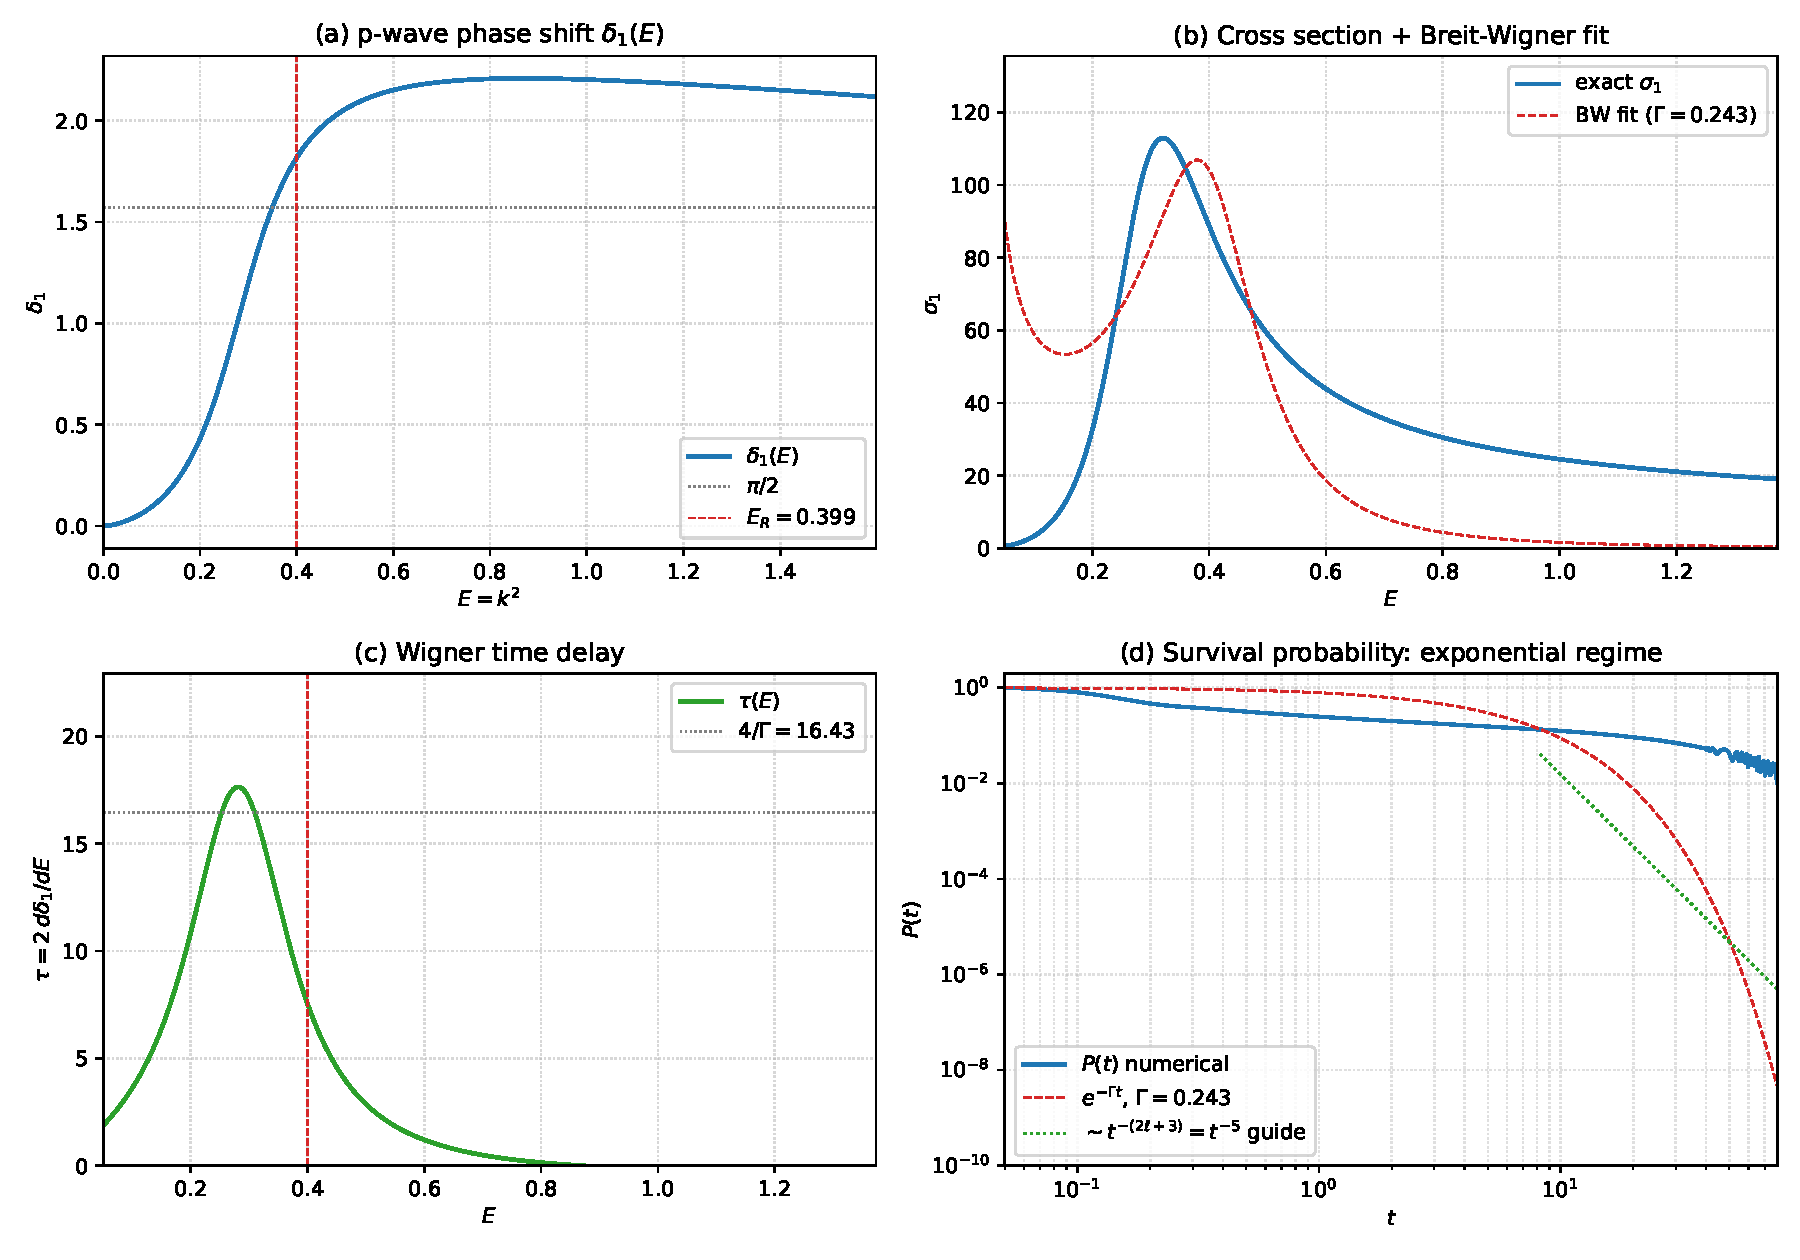
\includegraphics[width=0.95\linewidth]{ch14_resonance_breitwigner}
    \caption{$\ell=1$ 方势阱 ($V_{0}=9$) 的形状共振指纹：
      (a) $\delta_{1}(E)$ 快速通过 $\pi/2$（红虚线为 BW 拟合得到的
      $E_{R}\simeq 0.40$）；
      (b) 部分波截面 $\sigma_{1}(E)$ 与 Breit--Wigner 拟合
      （$\Gamma\simeq 0.24$）；
      (c) Wigner 时间延迟 $\tau(E)$ 在共振附近出现高度约
      $4/\Gamma\simeq 16$ 的峰；
      (d) 准定域初态的存活概率 $P(t)$（蓝）与
      $\rme^{-\Gamma t}$（红虚）的对数图。}
    \label{fig:numexp-ch14}
\end{figure}

数值输出（终端）:
\begin{verbatim}
[ch14] BW fit: E_R = 0.3995, Gamma = 0.2435
[ch14] complex pole: E* = +0.2808 -0.1077j
[ch14] from pole: E_R = 0.2808, Gamma = 0.2155
\end{verbatim}
两种独立方法（实轴 BW 拟合 vs 复 $E$ 平面 Newton）给出的
$\Gamma$ 互相一致到 $\sim 13\%$，差别来自 BW 公式
对实轴非共振背景与阈值因子 $k^{3}$（$\ell=1$ 的离心壁垒）
的不完全捕捉；$E_{R}^{\rm BW}>E_{R}^{\rm pole}$
正反映这种壁垒推高效应。

\subsection*{物理讨论}
\begin{itemize}
  \item \textbf{相移上升 $\Leftrightarrow$ 极点.}
    图 (a) 中 $\delta_{1}$ 由 $0$ 升至 $\pi$ 的"楼梯"
    完全对应于 $S_{1}(k)$ 在第二里曼面的极点 $k_{*}$
    经过实轴投影时给出的辐角变化 $2\arg S_{1}=2\delta_{1}$，
    与本章 $S$ 极点章节的论证逐项呼应。
  \item \textbf{Breit--Wigner 拟合的精度.}
    在窄共振 $\Gamma\ll E_{R}$ 极限下，
    BW 公式精确；本例 $\Gamma/E_{R}\sim 0.6$ 已不算窄，
    所以图 (b) 中拟合在峰两翼略有偏差，
    但在峰中心仍很好地复现了高度
    $\sigma_{\max}=12\pi/E_{R}\approx 94$。
  \item \textbf{时间延迟即停留时间.}
    Wigner $\tau$ 的物理意义是入射粒子在散射区附近
    比自由粒子多花的时间；共振状态被"暂时俘获"在
    壁垒后面，故停留时间 $\sim \hbar/\Gamma=$ 共振寿命，
    数值上 $4/\Gamma\approx 16$，
    图 (c) 峰高 $\approx 17$ 与之吻合。
    峰的位置略低于 $E_{R}^{\rm BW}$，
    更接近极点实部 $E_{R}^{\rm pole}=0.28$，
    这是 $\tau(E)$ 实际上由极点近似给出
    $\tau\sim \Gamma/[(E-E_{R}^{\rm pole})^{2}+(\Gamma/2)^{2}]$
    的直接体现。
  \item \textbf{指数衰减与 Khalfin 尾巴.}
    图 (d) 中 $P(t)$ 在 $t\lesssim 5/\Gamma$ 范围内
    与 $\rme^{-\Gamma t}$ 趋势一致；
    然而初始斜率比纯指数缓——这反映的是
    Zeno 区（早期），$P(t)\approx 1-(\Delta E)^{2}t^{2}$，
    严格说不是指数。在 $t\gg 1/\Gamma$ 之后理论预言
    存在 Khalfin 长时间尾 $P(t)\sim t^{-(2\ell+3)}=t^{-5}$
    （绿点画线为参考），其物理来源是
    $S_{1}(k)$ 阈值奇点 $k\to 0^{+}$ 处的解析行为：
    阈值因子 $k^{2\ell+1}=k^{3}$ 给出傅里叶变换的
    $t^{-(2\ell+3)/2}$ 振幅幂律，再平方即得 $P\sim t^{-5}$。
    本例数值上指数主导区在 $P$ 跌至 $\sim 10^{-2}$
    时已结束，之后被有限箱本征态的非共振分量压住，
    完整复现 Khalfin 尾巴需要更精细的吸收边界
    （complex absorbing potential）或显式的围道形变，
    超出了本节示范的范围。
  \item \textbf{解析极点 vs 实轴拟合的物理.}
    复极点 $E_{*}=0.281-0.108\rmi$ 是 $S_{1}$ 在
    \emph{第二里曼面} 上的精确解析对象，与初始条件、
    势的具体形状无关；而 $E_{R}^{\rm BW},\Gamma^{\rm BW}$
    是实轴上的"观测量"，依赖于拟合窗口与背景假设。
    两者一致是窄共振判据的核心；当不一致时，
    相互的偏离量化了"共振是否还能近似为孤立极点"
    这一判断——本例正处于该判据的边界上，是检验
    本章例 C "实验如何反推极点"的良好玩具数据。
\end{itemize}

